\section{Co-diseño con la política final de tendencia lenta}
% Generado por tools/resumir_codisenio_lento.py
\newcommand{\TablaFinalRecursos}{Software & 1087 & 1199 & 8 & 50,71 & PASS \\
Custom-0 & 1258 & 1368 & 10 & -- & FAIL \\
MMIO incremental & 1104 & 1219 & 9 & 50,67 & PASS \\
MMIO barrido & 1109 & 1227 & 9 & 51,04 & PASS \\}
\newcommand{\TablaFinalRendimiento}{Software & 127,07 & 303 & 55,04 & 2,31 & 24,24 & 98368,81 \\
Custom-0 & 125,07 & 303 & 54,04 & 2,31 & 24,24 & 99941,56 \\
MMIO incremental & 83,98 & 259 & 35,94 & 2,34 & 20,72 & 148847,90 \\
MMIO barrido & 83,98 & 259 & 35,94 & 2,34 & 20,72 & 148847,90 \\}
\newcommand{\TablaFinalRegiones}{Software & 11,50 & 7,13 & 49,10 & 59,34 & 21,10 \\
Custom-0 & 11,50 & 7,13 & 47,10 & 59,34 & 20,10 \\
MMIO incremental & 11,51 & 7,13 & 6,00 & 59,34 & 2,00 \\
MMIO barrido & 11,51 & 7,13 & 6,00 & 59,34 & 2,00 \\}
\newcommand{\TablaFinalAmdahl}{Software & 1,00 & 1,00 & 1,00 & 0,00 \\
Custom-0 & 1,04 & 1,02 & 1,02 & 0,00 \\
MMIO incremental & 8,18 & 1,51 & 1,51 & 0,01 \\
MMIO barrido & 8,18 & 1,51 & 1,51 & 0,01 \\}
\newcommand{\FraccionKernel}{38,64}

Se comparan cuatro implementaciones de SUM10 manteniendo exactamente la política
128/5\%, cartera causal, comisiones y ocho entradas de 20\,000 precios.
Cada implementación arranca desde cero. El banco estricto instrumentado conserva
las comprobaciones de MISO, DECISION, registros, cartera y plazo; además compara
SUM10 y READY en los registros CPU al terminar el kernel, incluso en software.
Son 32 ejecuciones y 640\,000 ticks; son cuatro implementaciones de los mismos
datos, no nuevas muestras financieras. Todas reproducen las mismas 98 compras,
92 ventas y patrimonios por conjunto de ocho series.

\subsection{Alternativas y método}
\textbf{Software:} historial circular, suma y contador en RAM; actualización
$S\leftarrow S-p_{viejo}+p_{nuevo}$ con instrucciones RV32E ordinarias. Es una
base incremental optimizada, no una suma ingenua de diez elementos por tick.
\textbf{Custom-0:} la misma base sustituye SUB+ADD por
\texttt{smaupd rd,rs1,rs2}, con $rd\leftarrow rd-rs1+rs2$ módulo $2^{32}$ y
tercer puerto de lectura. Se conserva el resto del kernel.
\textbf{MMIO incremental:} periférico activo, historial en BRAM y actualización
de suma en un ciclo; CPU lee SUM10 y READY. \textbf{MMIO barrido:} segunda
alternativa hardware, con igual interfaz y firmware, suma los precios válidos
del historial en hasta nueve ciclos. Completa antes de que la CPU solicite el
resultado. No cambia la decisión ni su significado temporal.

Los programas tienen 163, 162, 130 y 130 palabras, respectivamente. Las variantes
están aisladas en \path{proyecto4/alternativas/codisenio_lento/}; las fuentes
activas y el BIN no cambian. La instrucción personalizada recupera ALU y
decodificación del estudio histórico, con procedencia en el manifiesto, pero
todas las cifras de esta sección son nuevas mediciones de la política final.

Se usan Go Board HX1K/VQ100, mismo PCF, entrada 25 MHz, CPU 12,5 MHz, nextpnr
con semilla 1 y restricción 25 MHz. Fmax es el valor enrutado del dominio SoC;
la comparación de ciclos se ejecuta siempre a 12,5 MHz. El fallo de capacidad
no tiene Fmax válido ni imagen programable.
\begin{center}\small\begin{tabular}{lrrrrl}\toprule
Variante & LUT4 & LC & BRAM & Fmax (MHz) & Ruta \\\midrule
\TablaFinalRecursos\bottomrule\end{tabular}\end{center}

\subsection{IC, CPI, tiempo y capacidad de servicio}
La ventana va de recepción completa a escritura DECISION. IC cuenta
instrucciones retiradas dentro de esa ventana; CPI global es ciclos acumulados
divididos por IC acumuladas. Se promedian las ocho series de igual longitud.
Una operación útil en esta comparación es procesar un precio hasta DECISION,
independientemente de comprar, vender o mantener. La capacidad es
$12{,}5\cdot10^6/\overline C$ ticks/s, sin incluir espera de nuevas entradas;
la entrada real del ensayo es 10\,000 ticks/s. No significa órdenes bursátiles/s
ni una prueba a esa tasa máxima de servicio.
\begin{center}\scriptsize\begin{tabular}{lrrrrrr}\toprule
Variante & Ciclos medios & Máx. & IC media & CPI & Máx. ($\mu$s) & Ticks/s \\\midrule
\TablaFinalRendimiento\bottomrule\end{tabular}\end{center}
Los máximos son observados sobre estas series, no cotas formales. Las cuatro
variantes cumplen el período de 100 microsegundos en simulación, incluso contando
la trama y sincronización; Custom-0 sigue siendo inviable por área.

\subsection{Perfil regional y Amdahl}
Se separan cuatro intervalos consecutivos: recepción a lectura PRICE (RX),
actualización de cartera hasta inicio de kernel, kernel SUM10 hasta resultado
en registros y decisión hasta escritura MMIO. Su suma se comprueba por tick.
La frontera del kernel se identifica por PC del Assembly; incluye historial,
contador y puesta a disposición de SUM10/READY, no solo las dos operaciones
aritméticas. En MMIO comprende la recogida del resultado del periférico.
\begin{center}\small\begin{tabular}{lrrrrr}\toprule
Variante & RX & Cartera & Kernel & Decisión & IC kernel \\\midrule
\TablaFinalRegiones\bottomrule\end{tabular}\end{center}
En software el kernel ocupa \FraccionKernel\% de los ciclos medios. Se aplica
el perfil para identificar el trabajo acelerable: la decisión ocupa unos
59,34 ciclos (46,70\%) y el kernel 49,10 (38,64\%). SUM10 es un bloque
separable; tras acelerarlo, la decisión sigue dominando. Se aplica
Amdahl con $P=K_{SW}/C_{SW}$ y $S_K=K_{SW}/K_v$:
\[
S_A=\frac{1}{(1-P)+P/S_K},\qquad
S_{obs}=\frac{C_{SW}}{C_v},\qquad
\epsilon=C_v-(C_{SW}-K_{SW}+K_v).
\]
\begin{center}\small\begin{tabular}{lrrrr}\toprule
Variante & $S_K$ & $S_A$ & $S_{obs}$ & $\epsilon$ (ciclos) \\\midrule
\TablaFinalAmdahl\bottomrule\end{tabular}\end{center}
El residuo conserva las diferencias de sondeo y fase de recepción fuera del
kernel; no se fuerza igualdad con la predicción. La cartera y la política
permanecen en CPU y limitan el speedup total. Los cocientes comparan rendimiento
de implementación, no rentabilidad de estrategias distintas.

\subsection{Roofline y límites del modelo}
Para aislar SUM10 se cuentan operaciones aritméticas del indicador en régimen
estable: dos en software, Custom-0 e incremental; nueve sumas en barrido.
No se cuentan aquí direcciones ni control; el CSV conserva también
\texttt{alu\_kernel}, que sí incluye aritmética de direcciones. Se define
$R\leq\min(R_{pico},BI)$, con $I$ en operaciones del indicador por byte
del recurso limitante. Son techos arquitectónicos, no anchos de banda medidos.
El LSU de 32 bits admite como máximo 50 MB/s a 12,5 MHz; cada puerto BRAM de
historial de 16 bits admite 25 MB/s. Lectura y escritura BRAM son independientes.

\begin{center}\small\begin{tabular}{lrrrr}\toprule
Variante & Bytes/tick & $I$ & Techo memoria & Techo cómputo \\
 & recurso limitante & op/B & M op/s & M op/s \\\midrule
Software & 28 LSU & 0,0714 & 3,57 & 6,25 \\
Custom-0 & 28 LSU & 0,0714 & 3,57 & 12,50 \\
MMIO incremental & 8 LSU & 0,2500 & 12,50 & 25,00 \\
MMIO barrido & 18 lectura BRAM & 0,5000 & 12,50 & 12,50 \\\bottomrule
\end{tabular}\end{center}
Software y Custom-0 realizan cuatro lecturas y tres escrituras de 32 bits por
kernel estable; los primeros diez ticks añaden la inicialización del contador.
Incremental recoge dos registros de 32 bits, con una lectura y una escritura
lógicas de 16 bits en historial por actualización. Barrido recoge los mismos
dos registros, pero lee nueve valores de 16 bits y escribe uno. Su límite de
lectura BRAM es más restrictivo que el de recogida CPU.
Los techos CPU suponen al menos dos ciclos por instrucción aritmética; Custom-0
fusiona dos operaciones. Incremental dispone de resta y suma combinacionales;
barrido usa un sumador por ciclo. La intensidad del barrido cuenta más trabajo
para obtener el mismo SUM10; no representa una mejora de trabajo útil.

La tasa aritmética observada de extremo a extremo se obtiene multiplicando
ticks/s de la tabla por 2, 2, 2 y 9, respectivamente. Queda muy por debajo de
los techos porque incluye cartera, control, esperas e instrucciones. El roofline
no modela esas latencias y no predice por sí solo el tiempo del tick. Los ciclos
y Amdahl son la comparación principal de aceleración útil. El BRAM incremental
mantiene su lectura habilitada continuamente en el RTL activo: las operaciones
lógicas contadas no acreditan menos conmutación ni ahorro energético. No se
midió potencia.

\begin{center}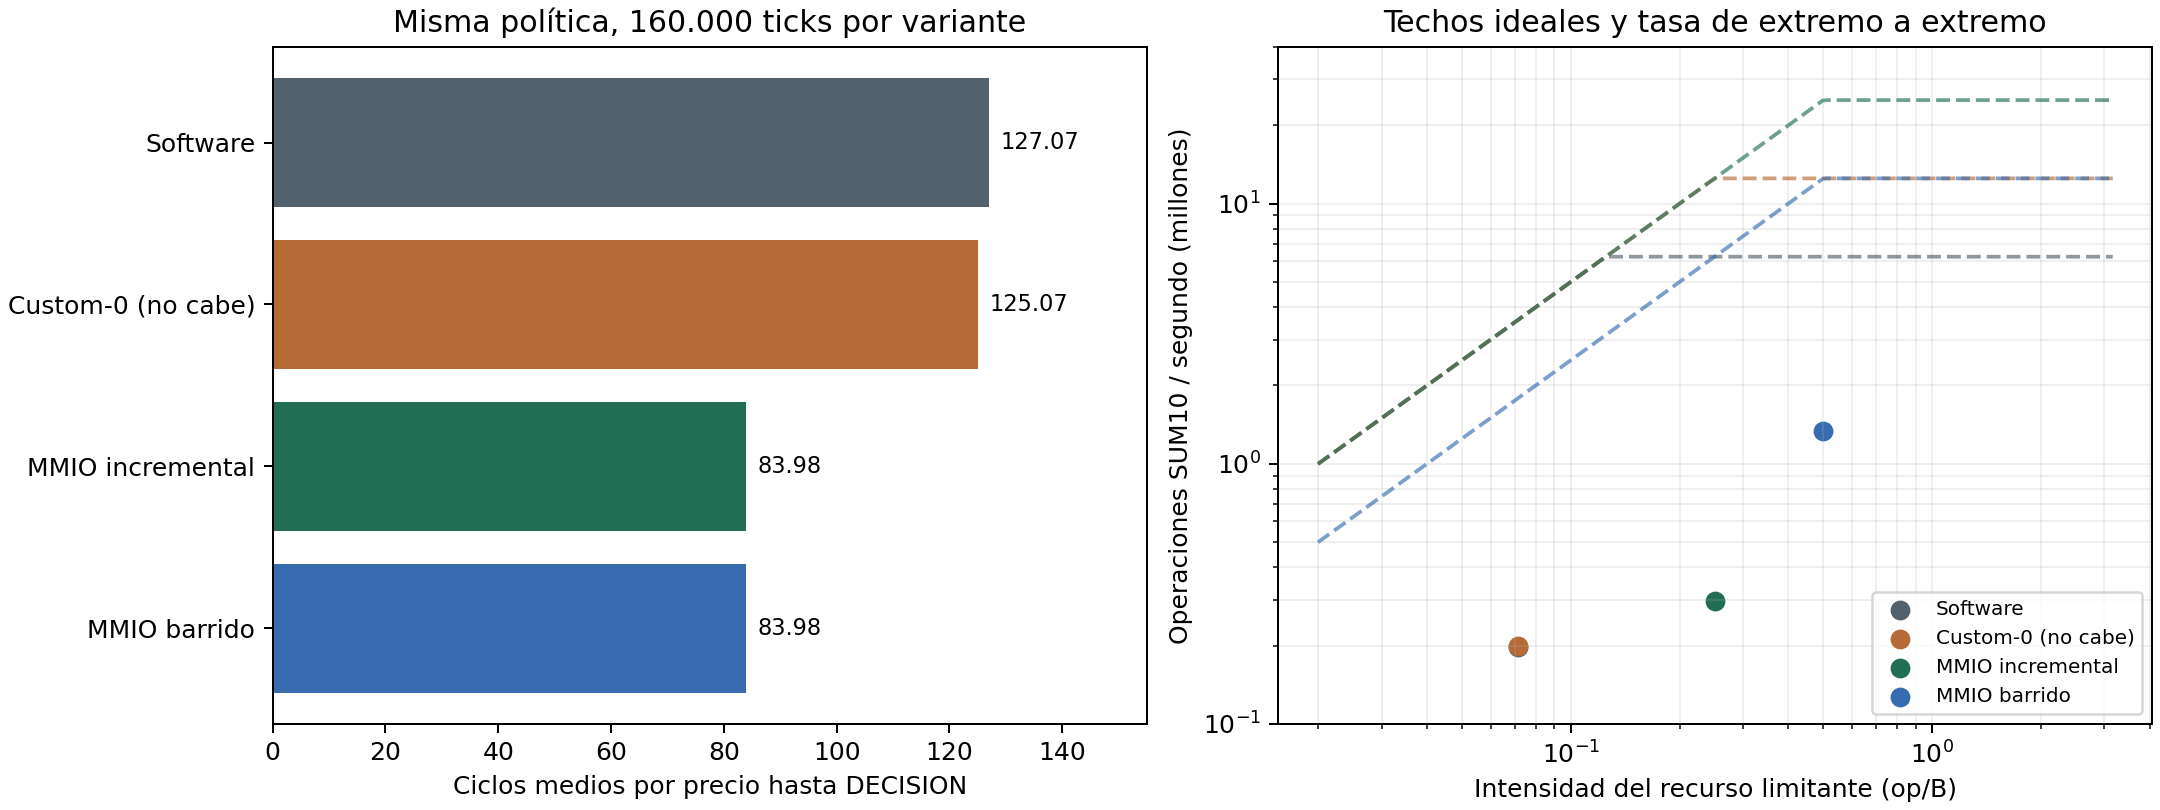
\includegraphics[width=\linewidth]{figuras/codisenio_final.png}\end{center}
Las curvas discontinuas son los techos ideales anteriores y los puntos son la
tasa aritmética derivada de las mediciones de extremo a extremo: 0,197; 0,200;
0,298 y 1,340 millones de operaciones SUM10/s. Software y Custom-0 casi se
superponen. El barrido ejecuta más sumas por el mismo resultado y tiene idéntica
capacidad útil que incremental; su punto más alto no significa mayor speedup.

\subsection{Elección y reproducción}
Se conserva \textbf{MMIO incremental}: cabe en la HX1K, reduce el kernel y
mantiene respuesta inmediata de SUM10. Barrido confirma una segunda aceleración
hardware viable, pero añade latencia interna y ocho LC frente a la imagen activa.
Custom-0 ahorra poco trabajo y su tercer puerto supera la capacidad de la placa.
No se cambia el BIN para obtener estas conclusiones.

Se archivan las 32 trazas completas comprimidas, hashes de fuentes, unidades,
netlists Yosys, logs y reportes nextpnr en
\path{docs/evidencia_codisenio_final/}. Las pruebas unitarias cubren 1024
vectores Custom-0, cinco codificaciones inválidas y 20\,040 precios por cada
periférico, incluyendo reinicio lógico sin borrar BRAM. La auditoría vuelve a
cotejar las 640\,000 filas contra los precios originales y modelo causal.
Los comandos, versiones exactas y resultados están en el README del repositorio.
